
\documentclass[12pt]{article} % use larger type; default would be 10pt

\usepackage[utf8]{inputenc} % set input encoding (not needed with XeLaTeX)

%%% PAGE DIMENSIONS
\usepackage{geometry} % to change the page dimensions
\geometry{a4paper} % or letterpaper (US) or a5paper or....
\geometry{margin=1in} % for example, change the margins to 2 inches all round
% \geometry{landscape} % set up the page for landscape
%   read geometry.pdf for detailed page layout information

\usepackage{graphicx} % support the \includegraphics command and options

% \usepackage[parfill]{parskip} % Activate to begin paragraphs with an empty line rather than an indent

%%% PACKAGES
\usepackage{booktabs} % for much better looking tables
\usepackage{array} % for better arrays (eg matrices) in maths
\usepackage{paralist} % very flexible & customisable lists (eg. enumerate/itemize, etc.)
\usepackage{verbatim} % adds environment for commenting out blocks of text & for better verbatim
\usepackage{subfig} % make it possible to include more than one captioned figure/table in a single float
% These packages are all incorporated in the memoir class to one degree or another...

%%% HEADERS & FOOTERS
\usepackage{fancyhdr} % This should be set AFTER setting up the page geometry
\pagestyle{fancy} % options: empty , plain , fancy
\renewcommand{\headrulewidth}{0pt} % customise the layout...
\lhead{CS 5150 Milestone 2 Report}\chead{}\rhead{Sun in the City Group}
\lfoot{}\cfoot{\thepage}\rfoot{}

%%% SECTION TITLE APPEARANCE
\usepackage{sectsty}
\allsectionsfont{\sffamily\mdseries\upshape} % (See the fntguide.pdf for font help)
% (This matches ConTeXt defaults)

%%% ToC (table of contents) APPEARANCE
\usepackage[nottoc,notlof,notlot]{tocbibind} % Put the bibliography in the ToC
\usepackage[titles,subfigure]{tocloft} % Alter the style of the Table of Contents
\renewcommand{\cftsecfont}{\rmfamily\mdseries\upshape}
\renewcommand{\cftsecpagefont}{\rmfamily\mdseries\upshape} % No bold!

%%% END Article customizations

%%% The "real" document content comes below...

\title{CS 5150 Milestone 2 Report \\ Sun in the City Group}
\author{Phillip Tischler (pmt43), Brian Toth (bdt25), Vera Khovanskaya (vdk9), \\ 
Sean Salmon (ss2669), Lin Xue (lx39), Zach Porges (zip2),  \\
and James McGuinness (jrm369)}
%\date{} % Activate to display a given date or no date (if empty),
         % otherwise the current date is printed 

\begin{document}
\maketitle
\tableofcontents
\clearpage

%%%%%%%%%%%%%%%%%%%%%%%%%%%%%%%%%%%%%%%%%%%%%%%%%%%%%%%%%%%%%%%%%%%%%%%%%%%%%%%%
\section{Milestone Summary}

Our team is about where we wanted to be for Milestone 2. Our project is to create a new website for The Cornell Daily Sun to expand their newspaper to the NYC Tech Campus. We have analyzed the market that the new website will compete in, considered tradeoffs for various designs, considered the various actors who will interact with the website and their use cases, designed layouts for the site, created an initial website and deployed to developmental servers, and started work on the Data Fusion Algorithm and Drupal Extension code. 

%%%%%%%%%%%%%%%%%%%%%%%%%%%%%%%%%%%%%%%%%%%%%%%%%%%%%%%%%%%%%%%%%%%%%%%%%%%%%%%%
\section{Project Description}

The goal of the project is to create a new website and Content Management System (CMS) for the Cornell Daily Sun in a new market: Cornell’s new Tech Campus in New York City. According to the client, Joseph Staehle, IT Manager for the Daily Sun, it should be a ``Totally online, totally tech based newspaper for the tech campus.”

The website is being built using Drupal, but will involve a custom front-end design as well as intelligent back-end technology. The website will include data fusion, aggregation of articles from other news sources.

%%%%%%%%%%%%%%%%%%%%%%%%%%%%%%%%%%%%%%%%%%%%
\subsection{Scope \& Requirements}

The project analyzed in this document is one to build a new website and Content Management System (CMS) for The Cornell Daily Sun. This website will represent a new market for the client. That is, the client is attempting to expand its newspaper to begin bringing news to the students of Cornell University’s new Tech Campus in New York City.
                   
\subsubsection{System Status}
                   
The Cornell Daily Sun website is an existing product that is managed with a Drupal CMS and custom extensions. This project is to build a new website for the Cornell Tech Campus, and is therefore a new product and not an augmentation or replacement. However, if this new website is extremely successful the old website may be converted to the new one. To maintain familiarity with the CMS system, the client has requested the CMS be based on the Drupal CMS.
                   
\subsubsection{Functionality}
                   
There are four required pieces of functionality the project must support: a website for readers to browse the newspaper, a CMS to manage the website and allow writers to post content, a means to allow Data Fusion to present external content inline with content generated by The Cornell Daily Sun, and finally a Brand to associate with this new website. Like the existing CMS The Cornell Daily Sun uses, the CMS must allow the writers and editors to upload their content like articles, blogs, comments, images, and advertisements. The website itself must display this content in a reasonable and convenient way that allows readers to browse and obtain the information they are looking for. To create a unique Cornell Tech campus newspaper, the project also requires the team to create a Brand. This includes a logo, a display name, and a look and feel for this newspaper. A key aspect of this Brand will be Data Fusion, a distinction from the current website the client operates. Data Fusion will present articles from external sources inline with an article posted by the Cornell Daily Sun. It is similar to a ``Read More" link, except this information will be external and automatically presented with the article from The Cornell Daily Sun.
                   
There are three desired but not required pieces of functionality for the project: an optimized mobile version of the site, an algorithm to perform the Data Fusion automatically, and a performance optimizer for the entire system. The mobile optimized site will allow readers to browse The Cornell Daily Sun’s website on a mobile device in a much faster and convenient way than to load the main page onto a slower device with less screen display area. This functionality may require too much time to implement, which is why it is not a required portion of this project. The Data Fusion described in the paragraph above was a framework to allow custom algorithms to link external content as well as manually link content. The other piece of functionality that is not required is an algorithm to automatically detect and link external content to the content generated by The Cornell Daily Sun. This may involve web and RSS feed scraping as well as Machine Learning and other advanced topics. Due to the complexity of the functionality relative to the timeframe of the project, this functionality has been deemed not required. However, if implemented it will save time, make running the website easier, and increase the attractiveness to potential readers as it will dynamically update the site. The final desired but optional piece of functionality is a performance optimization that will decrease the time it takes to load the website. Using a 50Mbps connection (an average user only has access to a 2Mbps connection), the client’s current site takes over 5 seconds to load the visible page of the homepage and over 13 seconds to load the entire page. Most websites can respond in under 200 milliseconds and load completely in a second. Every millisecond the user waits has a psychological impact on their perception of the website, and thus it is critical to load as fast as possible. There are simple upgrades to the system that can be employed to achieve this goal. However, time and budget may be a limiting factor, which is why this functionality is desired but not required.

\subsubsection{Dependencies}
                   
Drupal. Drupal is an open-source CMS that The Cornell Daily Sun uses for their current website, and as such the CMS that will be used for this project. The Drupal CMS is licensed under the GNU General Public License. This license is explained under the discussion of business considerations. Drupal is composed PHP, HTML, and CSS to generate and display the content, and a MySQL database to store the information composing the content itself. Drupal 6 requires PHP 4.4.0 or higher, while Drupal 7, the latest release, will be used and it requires PHP 5.2.5. Drupal provides a large baseline of features for a website, including but not limited to, user account handling, layout management, website menu customization, RSS feed aggregation, article search, and FTP access. Extensions can be written for Drupal in PHP, and there are over 17,000 free extensions available that are also under the GNU General Public License. For this project, Drupal will provide a very strong base for building this system.
Deployment Server. We will be using a Linux-based server hosted on a cloud platform for purposes of development and eventually deployment. The plan is to use Amazon AWS as the cloud provider. Because Drupal uses PHP and MySQL only, a Linux server is appropriate.
Data Fusion. The Data Fusion extension will most likely be integrated into Drupal using a PHP module, but the core functionality of the scraper will be written in Java. Because Drupal already has RSS aggregation, it is very likely that the module will rely on some form of RSS news scraping to find similar news articles.
Apache Lucene. The Data Fusion algorithm will be using the Apache Lucene indexing and search library that is licensed under the Apache 2.0 license. This license has been vetted and determined appropriate for this project.
                    

%%%%%%%%%%%%%%%%%%%%%%%%%%%%%%%%%%%%%%%%%%%%
\subsection{Benefits}

There are two unique stakeholder entities that will benefit this project. The first is The Cornell Daily Sun that will own the product that results from the project. The second is the students and other community members of Cornell University’s new Tech Campus. Each entity will benefit in different ways from the success of this project.
                   
\subsubsection{Cornell Daily Sun}
                   
With the new website, The Cornell Daily Sun will both expand its market, increase its influence, and increase its revenue. This project will allow the client to new types of content for both its paper based and web based publications. As the website matures, the project will allow the client to attract new readers on the order of 80,000. As the website displays advertisements, there will be a new source of income for the Cornell Daily Sun. Finally, with the new content and new readers in the New York City area, the website is very likely to attract new advertisers.
                   
Another potential benefit of the project is the integration of new technology. That is, the current website the client runs is on an older Drupal 6 CMS whereas the new website will be built with Drupal 7. Our new design will better organize the website content, and eciency code will be used to improve the compiling time from minutes to seconds. The Drupal 7 has major improvements over the Drupal 6. They are enhanced security (for scheduled tasks, password, and log-in), usability (better support for both administrators and users), and performance (new features for search, file handling, and RSS feeds). These new technical improvements are desired in the current Cornell Daily Sun website. If this project is a success, it can be deployed to replace the current website as well.
                   
\subsubsection{The Cornell Tech Campus Community}
                   
The website to be developed provides a way for broadcasting current news about the Cornell NYC Tech campus, which serves the Tech campus members and the general Cornell community. With blog services in addition to news, the website also enables individuals to share information with the community about tech topics, their life, campus life, alumni activity, and career experience. 

%%%%%%%%%%%%%%%%%%%%%%%%%%%%%%%%%%%%%%%%%%%%%%%%%%%%%%%%%%%%%%%%%%%%%%%%%%%%%%%%
\section{System Design}

The system has been designed to be as modular and uncoupled as possible. The Cornell Daily Sun’s current website is highly coupled and has prevented them from upgrading their system form Drupal 6 to Drupal 7.

The website will be hosted on Amazon AWS running an Apache 2 Web Server and a MySQL Database Server. Drupal 7 will be used to provided the base CMS and website structure. The team will develop custom XHTML, CSS, and PHP to create a ``theme" in Drupal. This customization can easily be ported to other Drupal versions and is a lightweight display layer. This will generate the viewable site and handle HTTP requests.

\begin{figure}[htbp]
\begin{center}
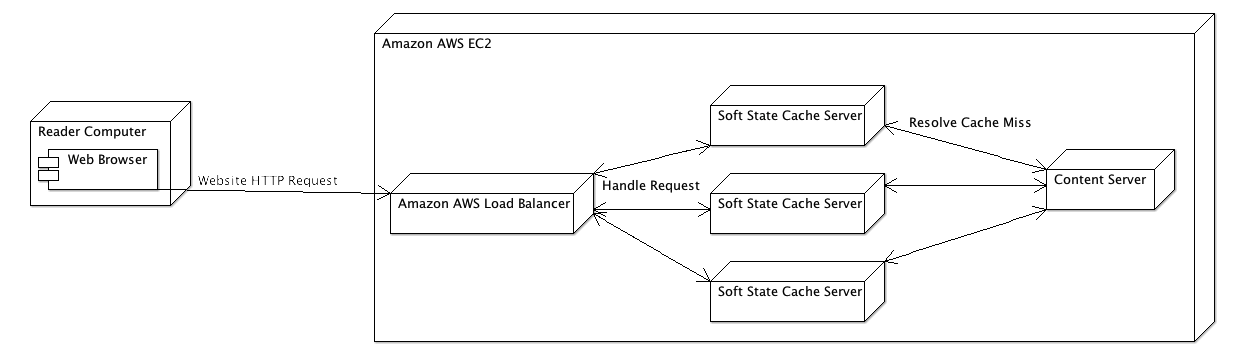
\includegraphics[width=6in]{images/data_flow}
\caption{Deployment Diagram}
\end{center}
\end{figure}

A Varnish server will be used as a soft-state in memory cache server. It works as a reverse proxy HTTP server and can handle about 3,000 page requests a second. This will provide incredible performance and scalability of the new site. Drupal also has pre existing modules to integrate with Varnish. This allows Drupal to invalidate page cache entries as the website is updated by The Cornell Daily Sun and happens completely behind the scenes.

Java will be used for the Data Fusion algorithm. The first component is RSS and Website Feed scraping. Various libraries are being analyzed to handle this workload. Essentially, the program will listen to RSS feeds and store the data in a MySQL database. Another component, the indexer, will take the data that has been scraped and put it into an Apache Lucene Index. Finally another component, the data fusion algorithm, will use the meta-tag taxonomy of an article to search for relevant data in the RSS and Website Apache Lucene Index, and store likely matches in another MySQL table.

To choose which Data Fusion articles get posted on the website, the team will build a lightweight PHP Drupal Extension to allow editors to approve fusion results as well as add in manual fusion data. This module will be an extremely lightweight and as decoupled as possible.

\begin{figure}[htbp]
\begin{center}
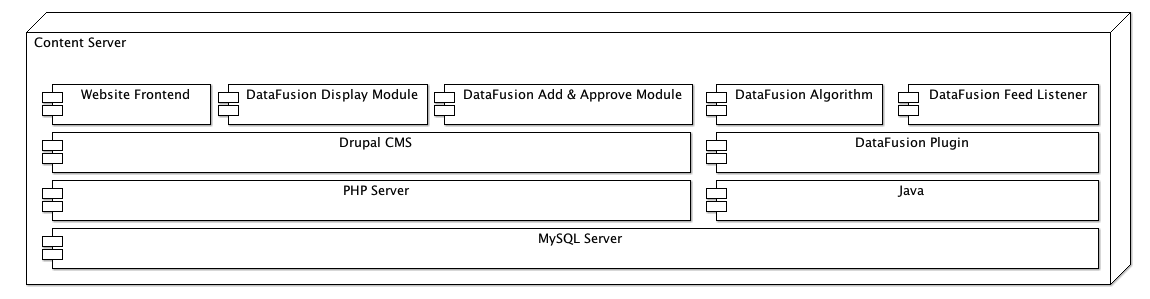
\includegraphics[width=6in]{images/software_stack}
\caption{System Architecture}
\end{center}
\end{figure}

%%%%%%%%%%%%%%%%%%%%%%%%%%%%%%%%%%%%%%%%%%%%%%%%%%%%%%%%%%%%%%%%%%%%%%%%%%%%%%%%
\section{Progress for Milestone 1}

%%%%%%%%%%%%%%%%%%%%%%%%%%%%%%%%%%%%%%%%%%%%
\subsection{Space Analysis}

The design process began with investigating prominent tech blogs and news websites. We reviewed eighteen sites in total, but the two sites that remained most relevant to use were the New York times Bits tech blog and The Verge. Other tech websites included Engadget, Gizmodo, and CNet. Our interest in doing this was to develop a design vocabulary, or a way of talking about our design process in a way that related to other, existing projects in the same space as ours.

%%%%%%%%%%%%%%%%%%%%%%%%%%%%%%%%%%%%%%%%%%%%
\subsection{Tradeoffs}

Specifically, we developed a design vocabulary that described each website in the ``space" we studied as a series of tradeoffs that were expressed in a website’s design. The trade-offs that we found most relevant are described below:
                   
\subsubsection{Designing for editorial control vs. popularity}
It is important for editors to control the news website, it should also be ``alive", generating content from across the web and from users. We noticed that some websites were heavily controlled by editorial staff (with categories such as ``featured selection" and ``editor’s picks" having visual prominence) and we noticed that other websites were instead controlled by popularity, and that most read articles appeared more prominently on the homepage. We intend to have a data fusion element which provides relevant articles, but editors must approve them. We will also allow users to comment on articles and will have some method for featuring the most popular posts.

\subsubsection{Blog content: tech hacker vs. tech curious}
While this was not a primary focus for us, we noticed that different sources appealed to different audiences: some websites were directed at people with significant pre-existing technical knowledge while others were aimed toward mainstream readers (with few assumptions about their existing knowledge). We decided that our content should appeal to ``hardcore nerds," but also to the general ``tech curious" public. We decided with our client that iIn order to maintain a broad audience and match the needs to the Tech Campus, articles will primarily be targeted towards the general public with an interest in tech, rather than just those who understand and appreciate hacking. Articles will also feature entrepreneurship, as this will be of interest to readers at the tech campus. We stress however, that these trade-offs in content were decisions that we made with the guidance of our client, and that they are somewhat out of our intended scope for the software engineering project.

\subsubsection{Dynamic vs. static data organization}
Some of the websites that we reviewed had several, nested menus that reflect various aspects of technical news. We felt as though these tended to get cumbersome as technical fields changed, and decided that the best way to handle this trade-off would be to allow some categories to be permanent, while others are temporary and change with trending topics. We will have permanent links on the homepage that filter articles by categories including news and entrepreneurship, but other links that can easily be modified by editors with trending tags.

%%%%%%%%%%%%%%%%%%%%%%%%%%%%%%%%%%%%%%%%%%%%
\subsection{Actors \& use Cases}

\textbf{Reader}. Readers are the consumers of both the primary and secondary content on the website. They will generate the bulk of trac to the system as there are orders of magnitude more readers as other types of actors. The use case they will primarily exercise is that of reading content on the website. They can find this content by either searching for it or browsing the various categories. It will be important to build trust with these users so that they desire to engage with the main content and with the secondary sources that we hope to integrate. Our own experiences with news content align most closely with this use-case, so we hope to accomplish preliminary usability testing on ourselves; however, as we grow more accustomed to the interface as developers, it will become increasingly important to test this use case on external audiences. This use case is of primary interest as it will define the success or failure of our client as these external stakeholders will generate the revenue.
                   
\textbf{Editor}. This is that actor that represents our clients, and is of high priority because they will have the most responsibilities and most investment when interacting with the system. Editors exercise the use cases of editing content posted by writers, determining which content should be posted to the website, and approving the Data Fusion sources. Editors are the executors of the newspaper’s broader vision, and the intermediaries between the writers and the users. Editors will also need to understand how to maintain the system, and will be particularly sensitive to the various data fusion and machine learning algorithms the team may be implementing. It is important to consider the editors’ needs in usability testing because they are the ”keystone species” of this news content ecology.
                   
\textbf{Writer}. The writers are the actors that generate primary content for the website and then decides what kind of secondary data, like Data Fusion sources, to include in their specific contribution. The use cases that writers go through are important to test because these actors are likely to be the less familiar with the system as they are least invested with The Cornell Daily Sun, and yet the most tech-savvy of our three actors as they will be generating content for a newspaper that is technical in nature.

\textbf{Interview Analysis}. Our initial interview analysis was with potential authors for the paper; we spoke with two current Cornell Daily Sun blog writers to learn about their use of the existing web system and their expectations for the new system. We learned that current staff writers edit their articles in other collaborative writing platforms (namely, google docs) and often prefer to handle the passing over of their writing using email. They expressed concern that the existing system was cumbersome and that they lacked the knowledge and training to operate it, and were adamant about not being interested in learning. From this we concluded that the system that we build should be easy to learn but, in the event that our writers are not interested, that the essential editorial controls should be easy to handle by a third party (namely, the editors.)


%%%%%%%%%%%%%%%%%%%%%%%%%%%%%%%%%%%%%%%%%%%%
\subsection{Layout \& Initial Drupal Website}

The home page will contain a featured article at the top, and a grid of headlines below. The articles can be filtered by tag. This view will show more details, and will contain a list of all recent articles in the right column. There is also space in this column for ads and other content. Finally, the article view contains the consistent header and sidebar, but shows the full article and comments.

Zen, a simple Drupal theme for making custom sub-themes, was used as a starting point. The website has three views: the home page, a collection of articles with a common tag, and a news article.

More work needs to be done on styling the website, but the screenshots below show the current version of the website, and are based on the mockups above.

\begin{figure}[htbp]
\begin{center}
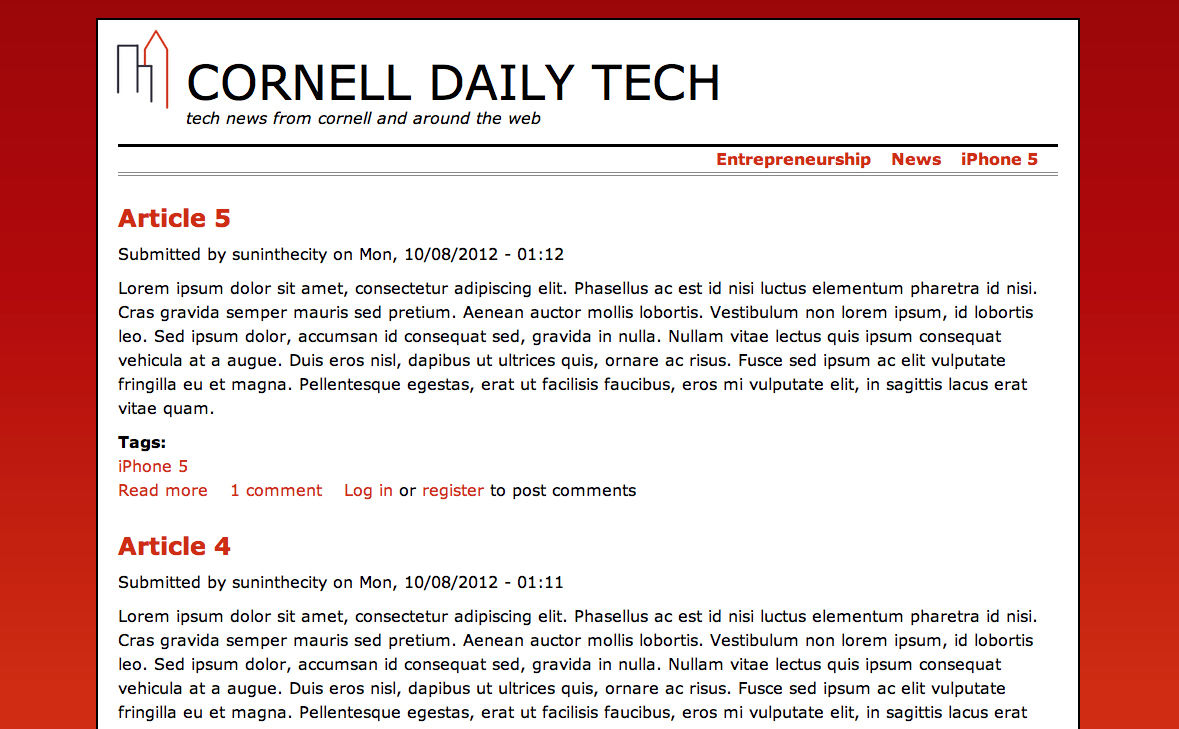
\includegraphics[width=3in]{images/web-main}
\caption{Initial Website: Homepage}
\end{center}
\end{figure}
This is a screenshot of the home page, but note that the formatting/design is still in its early stages. The top right section contains links to collections of articles with a common tag. This header is consistent across all pages on the website, and the links easily can be modified by an administrator.

\begin{figure}[htbp]
\begin{center}
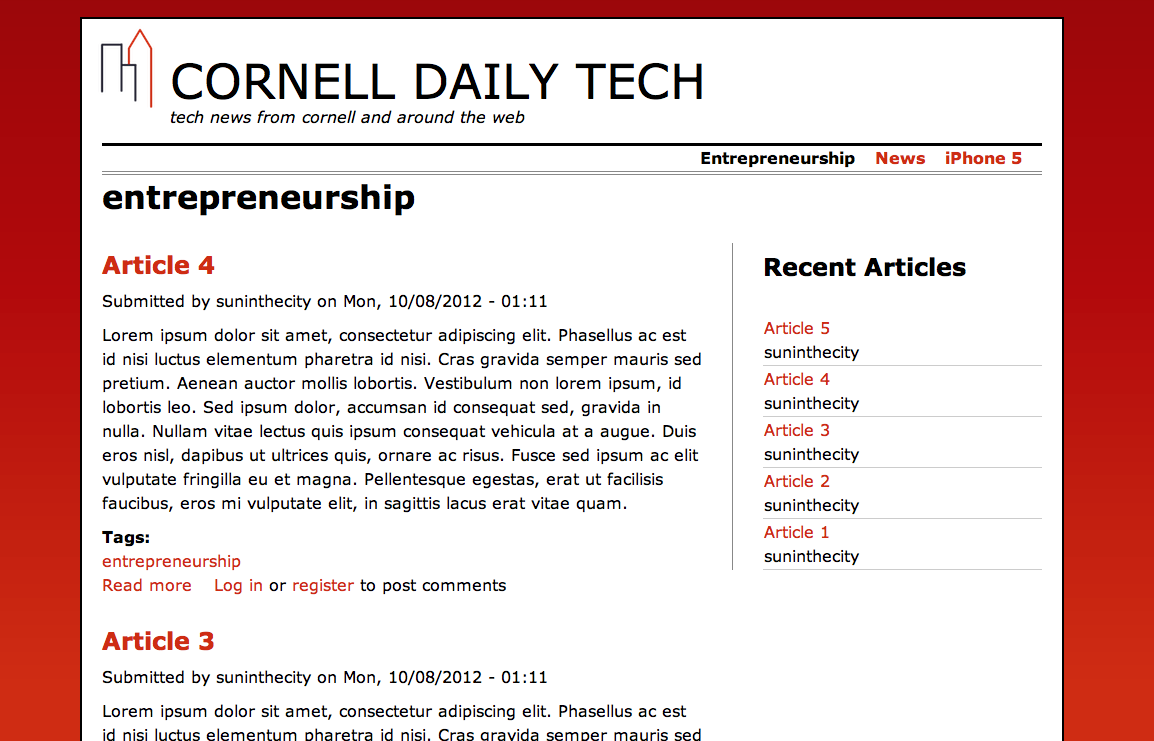
\includegraphics[width=3in]{images/web-topic}
\caption{Initial Website: Topic}
\end{center}
\end{figure}
This page shows all articles tagged with entrepreneurship. Note that the right column of this page, and all other pages except for the home page, contains links to articles that were recently published. There is additional space in this column for ads or other content.

\begin{figure}[htbp]
\begin{center}
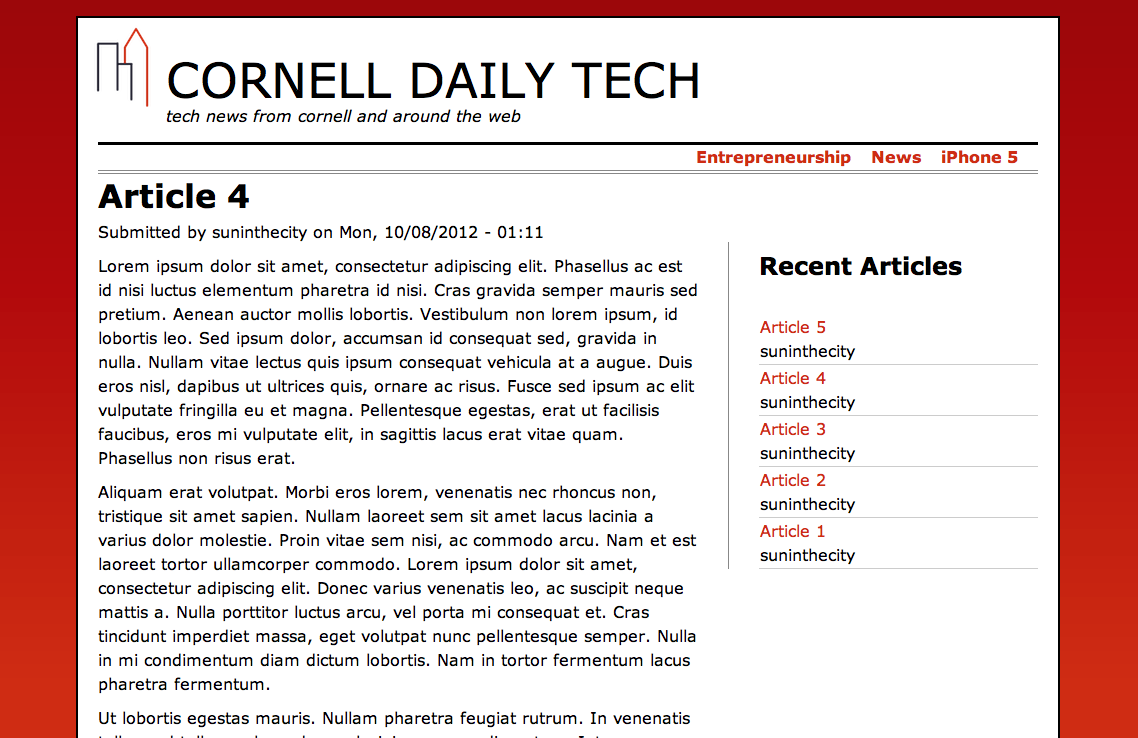
\includegraphics[width=3in]{images/web-article}
\caption{Initial Website: Article}
\end{center}
\end{figure}
Finally, this is the article view. Articles are easy for editors to add/modify using Drupal, and they contain Drupal’s commenting system.

%%%%%%%%%%%%%%%%%%%%%%%%%%%%%%%%%%%%%%%%%%%%
\subsection{Database Design}

The majority of the CMS database system is designed and maintained by Drupal. The portions we are working on are the backend for the RSS and Data Fusion algorithms. The tables are as follows: DataSource, DataMeans, DataPrimary, DataSecondary, and DataFusion. The DataSource table contains news sources like The New York Times. The DataMeans table contains content generators like The New York Times RSS Feed. DataPrimary table contains all the content generated by those feeds and DataSecondary contains linked sources from that. For example, the RSS feed may contain a link to the main article which would be stored in the DataSecondary table. Finally, there is the DataFusion table which stores the results of the algorithm as well as the manual data fusion operation.

\begin{figure}[htbp]
\begin{center}
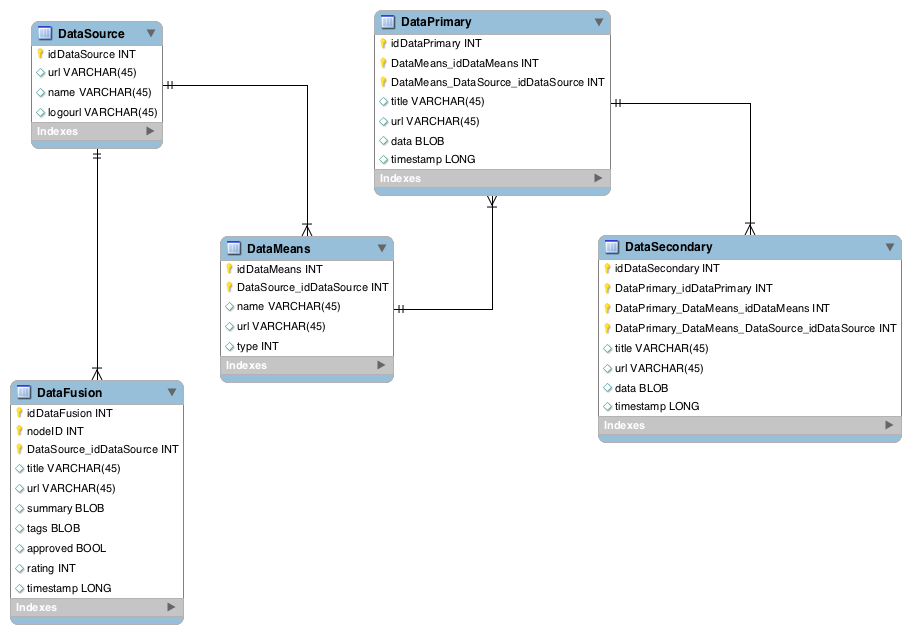
\includegraphics[width=6in]{images/database_model}
\caption{Database Model}
\end{center}
\end{figure}

%%%%%%%%%%%%%%%%%%%%%%%%%%%%%%%%%%%%%%%%%%%%
\subsection{RSS \& Web Scraping}

RSS feeds are used for gathering news sources and data for the Data Fusion algorithm, and ultimately for display on the website. RSS feeds can be added and managed. (More on the Drupal extension for managing RSS feeds here). The RSS feeds and their URLs are added to an SQL table in the server.

RSS and web scraping is handled within a Java package that utilizes both an SQL
connection API and an RSS aggregation API. Upon startup, the Java package reads a
set table that contains all of the URLs and identifiers for the RSS feeds that need to be
monitored. For sake of sanity and ensuring that no duplicate entries are created, only
RSS posts newer than the time of initialization will be analyzed. A basic Java SQL driver,
called JConnector (supplied by Oracle as part of the standard MySQL package, and licensed
under MySQL and the GNU General Public License) is used for reading and writing to SQL
tables as needed.

At startup, an object called SourceTable is created in order to initalize a connection
to the RSS source table and read from it. Calling a function getSources on this object
will retrieve a Set<NewsSource>, a set of NewsSources. This set will be added to using
a function called addSources after a cooldown of a couple of hours.

Upon reading any URL for a RSS feed from the server's database, it will be
initialized using a Java RSS Reading API called ROME, which supports any version of RSS
along with Atom. ROME is licensed under the Apache 2.0 license. ROME makes it easy to
retrieve the data of an RSS feed, along with the URL the RSS links to. Using a function
generateReader within the class NewsSource, a NewsReader will be generated inside of the
class. This will retrieve new RSS posts using ROME.

A ThreadPool will be running, and will use a Semaphore for signaling whenever a NewsSource
has a new post. The NewsSource class will have a function hasNewPosts, returning a boolean
of whether or not the RSS feed tied with the NewsSource has any new posts to read. If so,
the master thread will V on the Semaphore, signaling a thread in the ThreadPool to
read that NewsSource's new post. This will then be turned into an object called NewsData
using a function called createData, which will then be passed into the function
DestTable.writeData, where DestTable is an object containing an SQL connection to the
table(s) where the RSS News data will be written to. This is then read in by the Data
Fusion Algorithm.

\begin{figure}[htbp]
\begin{center}
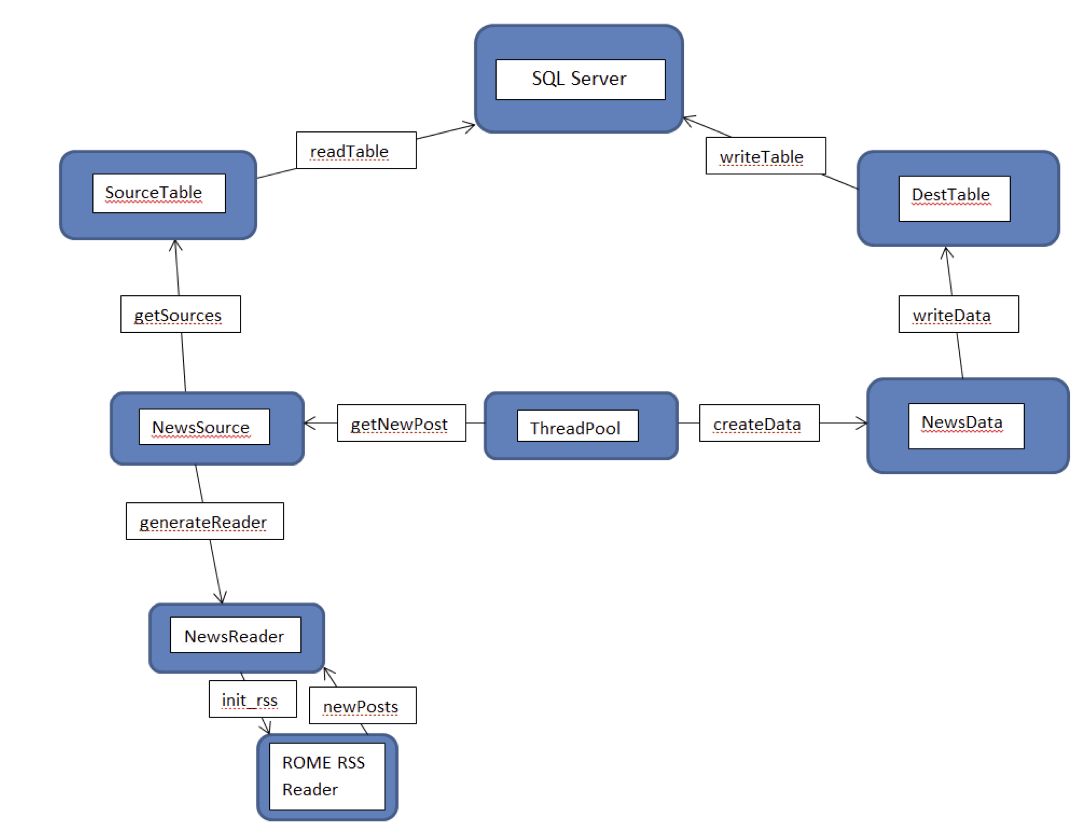
\includegraphics[width=6in]{images/rss_diag}
\caption{RSS Operation}
\end{center}
\end{figure}

%%%%%%%%%%%%%%%%%%%%%%%%%%%%%%%%%%%%%%%%%%%%
\subsection{Data Fusion Algorithm}

The Data Fusion algorithm has been designed to rely on existing proven systems. The algorithm will take data from various sources, like The New York Times articles, and insert them into an Apache Lucene index. Then for each Cornell Daily Sun article it will use the meta-tags (taxonomy) of the article to search the Apache Lucene Index for relevant articles. Finally, it will take the likely matches and insert them into the Data Fusion table.

\begin{figure}[htbp]
\begin{center}
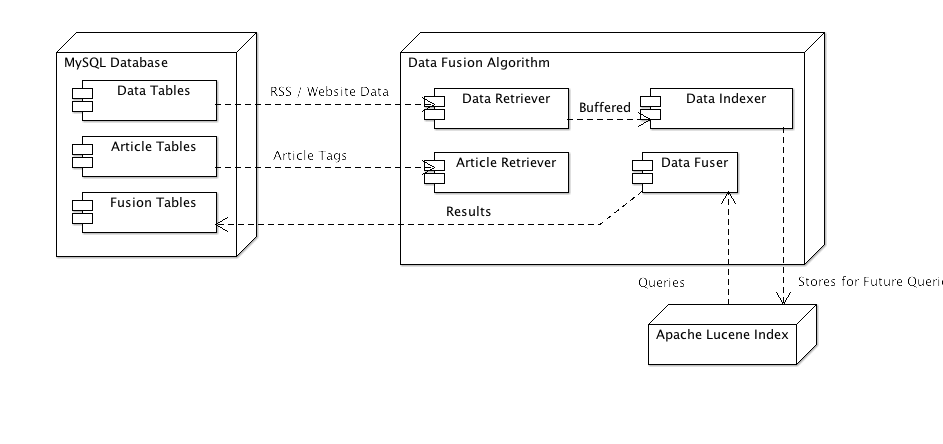
\includegraphics[width=6in]{images/data_fusion_alg}
\caption{Data Fusion Algorithm}
\end{center}
\end{figure}

For this milestone this structure and this library has been determined. A skeleton base code has been created and all that remains is coding and testing the algorithm. As Apache Lucene is one of the premier search systems, it is likely that this system will work to desired specifications.

%%%%%%%%%%%%%%%%%%%%%%%%%%%%%%%%%%%%%%%%%%%%
\subsection{Drupal Extensions}

The Drupal Extension will be used to edit the Data Fusion results as well as approve them to be shown on the website itself. The team has designed a prototype interface for this system as well as walked through its operation. We have also gone through example Drupal Extension code to understand how to interact with it.
       
\begin{figure}[htbp]
\begin{center}
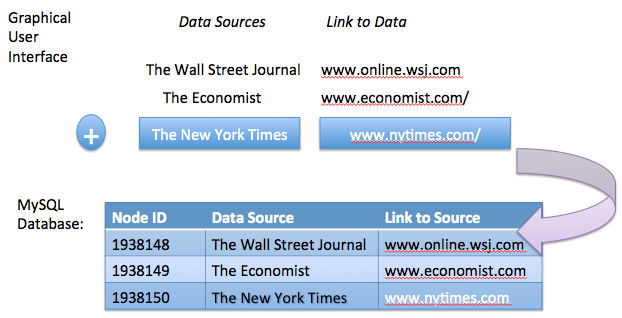
\includegraphics[width=6in]{images/drupal_ext_interface}
\caption{Example Drupal Extension Interface}
\end{center}
\end{figure}

%%%%%%%%%%%%%%%%%%%%%%%%%%%%%%%%%%%%%%%%%%%%%%%%%%%%%%%%%%%%%%%%%%%%%%%%%%%%%%%%
\section{Planning}

In terms of our original plan, we have deviated slightly from it. First, we originally planned to deploy our development system to an offsite development server provided by The Cornell Daily Sun. However, this fell through as we could not get access to their systems in time, so we decided to install individual development servers on everyone’s personal machine instead. Each person can receive changes by pulling from the git repository which includes the creation script (database dump) to setup MySQL. In addition, we also planned to have more concrete decisions on branding and ad placement on the site, but conversations are still ongoing with our client.

The rest of our plan we are on schedule with. For Milestone 3 we plan to have a full working system including RSS feed storage, Data Fusion algorithm, and Drupal extensions. For Milestone 4 we plan to be deployed to Amazon AWS, if possible have Elastic Cloud and Caching working, and have the entire system documented and handed over. 

%%%%%%%%%%%%%%%%%%%%%%%%%%%%%%%%%%%%%%%%%%%%%%%%%%%%%%%%%%%%%%%%%%%%%%%%%%%%%%%%
\section{Issues Arisen}

So far, no major issues have arisen. Initially, several team members struggled to install Drupal on their local machines. Different systems required LAMP, WAMP, MAMP, or XAMP. Issues involved user permissions, enabling Apache MODS, and rewriting URLs and Symlinks, but the issues were resolved.

%%%%%%%%%%%%%%%%%%%%%%%%%%%%%%%%%%%%%%%%%%%%%%%%%%%%%%%%%%%%%%%%%%%%%%%%%%%%%%%%
\section{Preliminary Documentation}

At this point of the project there are no custom systems built and therefore, only the integration of existing systems. Therefore, the only documentation necessary at this stage of the process are already written and maintained by external sources. They have been included below:

\begin{itemize}
\item https://help.ubuntu.com/community/ApacheMySQLPHP
\item http://drupal.org/documentation
\item http://lucene.apache.org/core/4\_0\_0/index.html
\item https://www.varnish-cache.org/docs
\end{itemize}

\end{document}
